\documentclass[11pt,a4paper]{report}
\usepackage[latin1]{inputenc}
\usepackage{amsmath}
\usepackage{amsfonts}
\usepackage{amssymb}
\usepackage{graphicx}
\usepackage{longtable}
\usepackage{multirow}% http://ctan.org/pkg/multirow
\usepackage{hyperref}
\usepackage{gensymb}
\usepackage{pdflscape}
\hypersetup{colorlinks=true,allcolors=black}
\usepackage{hypcap}
\usepackage{cleveref}
\usepackage{amsmath}
\usepackage[export]{adjustbox}
\usepackage{tikz}
\usepackage{tikz-qtree}
\usepackage{placeins}
\usepackage{array}
\usepackage{subcaption}
\usepackage{footnote}
\usepackage{color,soul}
\newcolumntype{L}[1]{>{\raggedright\let\newline\\\arraybackslash\hspace{0pt}}m{#1}}
\newcommand{\note}[1]{\marginpar{\tiny{ \hl{#1 } } }  }
\begin{document}

\begin{titlepage}
	\begin{center}
		\vspace*{-.5cm}
		\textsc{\LARGE Swinburne University of Technology}\\
		
		\begin{figure}[h]
			\centering
			
\includegraphics[width=0.5\linewidth]{swinburne_university_of_technology_111401}
		\end{figure}
		\vspace*{2cm}
		\hrule \  \\[0.4cm]
		\textsc{\Huge Hand-Eye Coordination Report}\\[0.5cm]
		\hrule \  \\[0.4cm]
		\textsc{\Large{RME 40003}\\ \  \\[0.1cm]
			\huge Robot System Design}\\[1cm]
		
		\normalsize\note{enter names and numbers}
		\begin{tabular}{l r}
			\hline\\ Justin Sargent & 00000 \\[0.25cm]
			\\ Phillip Smith & 7191731 \\ [0.25cm]
			\\ Thomas Rappos & 00000 \\[0.25cm]
			\hline 
		\end{tabular} 
	\end{center}
\end{titlepage}
\tableofcontents
\chapter{Project Outline}
This project explores the use of a robotic arm used for pick-and-place automation tasks. For dynamic operation and task-completion feed-back, computer vision is incorporated via a web-cam mounted in the work area.\\
More specifically, this project has been completed for an industry client, AME System Pty. Ltd., for automated cavity plug insertion. These plugs are 1.5mm\note{double check size} wide and are placed in cavities between 2 and 4mm apart. As such, a high degree of accuracy and repeatability is required. \note{include image of plug}
\chapter{Gripper Design}
With such small objects being handled, a custom gripper device was developed. The main gripper mechanism uses a Festo parallel, nematic gripper. While the gripping appendages have been custom made for this operation. Shown in \cref{fig:gripper2} are the open and closed CAD renderings of the gripper. Dark-grey being the Festo gripper, light grey being the main gripper appendage and green being the 3D printed gripper tips, modelled to specify grasp the cavity plugs.\footnote{two cavity plug sizes were initially requested}

\begin{figure}[h]
\centering
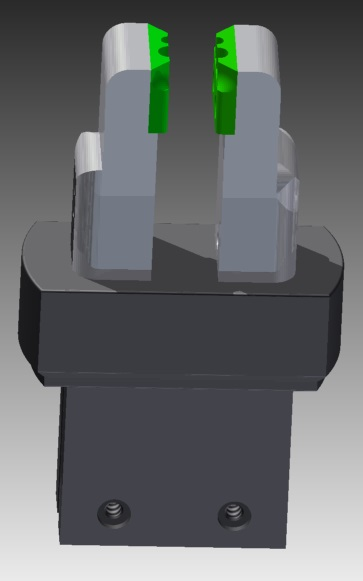
\includegraphics[width=0.4\linewidth]{gripper2}\ %
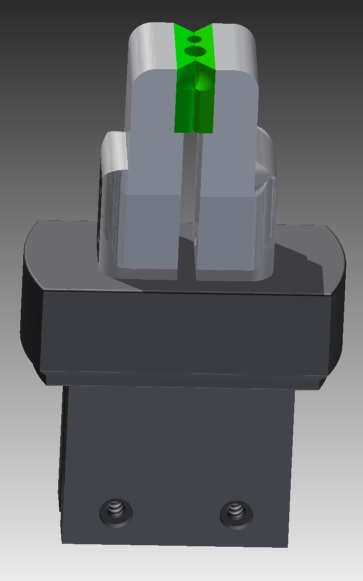
\includegraphics[width=0.4\linewidth]{gripper1}
\caption{CAD rendering of plug gripper}
\label{fig:gripper2}
\end{figure}


\chapter{Computer Vision}
The computer vision of this project uses Open-CV for c++. This library contains many image-based functions for sourcing, manipulating, and presenting visual data. This library has been used for two roles, object detention, and robotic gripper required motion determination. Of these two task, the latter relies on the former. 
\section{Object detection}
\subsection{Environment preparation}
To begin the computer vision process a background image is taken when no objects are present. A keyboard control was added, 'Y', which allows a new background to be set. This was seen to be useful, as a background image taken on start-up, would often be too bright. This was seen to be due to the automated settings of the camera not having finished calibrating.\\
With the background set, a psudo-live stream of stills was captured from the camera. Each of these stills was then processed, as follows, before being discarded. 
\subsection{Object recognition}
The first step of still processing was to do a raw matrix subtraction of the background. This gave an image of only the objects not in the background image. For this subtraction to function correctly, the background image needed to be free of all free-moving objects, as this subtraction would recognise a lack of object as well. An example of this subtraction is shown in \cref{fig:backgrond}.\\
\begin{figure}
	\hspace*{-0.1\linewidth}
	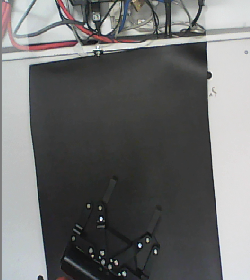
\includegraphics[width=0.6\linewidth]{backgrond} %
		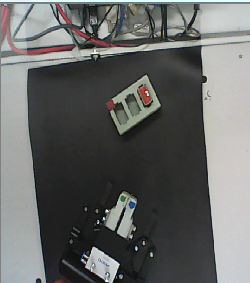
\includegraphics[width=0.6\linewidth]{base}\\
		\hspace*{0.2\linewidth}
			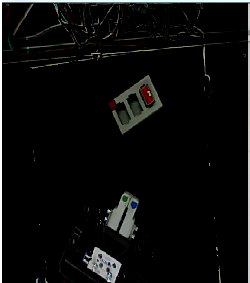
\includegraphics[width=0.6\linewidth]{diff}
	\caption{ Background image, new capture with objects in place and resulting subtraction }
	\label{fig:backgrond}
\end{figure} \
This image was then converted to a binary matrix, with a threshold of each colour layer, and a a grey scale process, to combine the colour layers. This process is shown in \cref{fig:out2}.\\ 
\begin{figure}
	\hspace*{-0.1\linewidth}
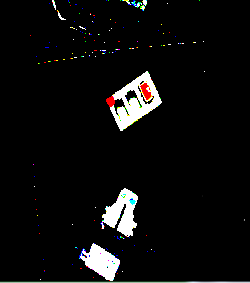
\includegraphics[width=0.6\linewidth]{out1} %
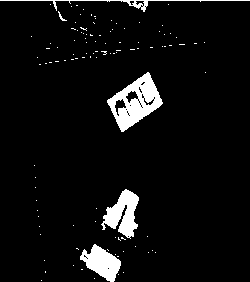
\includegraphics[width=0.6\linewidth]{out2}
\caption{Threshold of each colour, and combining of colour layers to make single layer binary}
\label{fig:out2}
\end{figure}
\begin{figure}
	\centering
	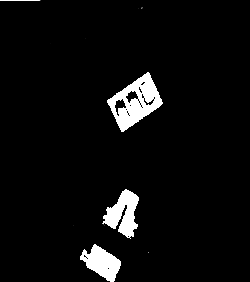
\includegraphics[width=0.6\linewidth]{out4}
	\caption{Erode and Dilate removes static from image}
	\label{fig:out4}
\end{figure}
\begin{figure}
	\centering
	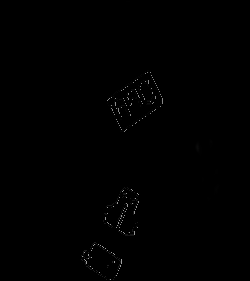
\includegraphics[width=0.6\linewidth]{out3}
	\caption{Canny edge detection leaves only the outline of the objects}
	\label{fig:out3}
\end{figure}
The resulting image was then eroded and dilated by one pixel layer. This erode function turns any white pixel touching to a black pixel into a black pixel, while the dilate function performs the opposite. This resulted in any small imperfections being removed from the image, while only slightly reducing the object recognition quality of the image. This is seen in \cref{fig:out4}.



A Canny edge detection was then used, which finds object edges by leaving only white pixels that are touching black pixels behind. The resulting image is shown \cref{fig:out3}.



Each group of remaining white pixels was now classified as a contour, via the \textit{findContours} command. This process found any collection of white pixels as a polygon shape. It also listed the contour hierarchy, where contours are set as parents, and any contours inside its pixel range are defined as its children. For the detection of the main holding box, and the gripper, which are at the highest level contour were wanted. Therefore, only contours with no parents were examined.\\

Each contour examined was fitted inside a rectangle with \textit{minAreaRect}. This found the smallest rectangle, of any angular orientation, that could fit the whole contour. The size of this contour was then tested, anything under or over a set threshold was removed.\\
For each rectangle that was within the size domain, a classification and orientation was attempted as a holding box. If this process failed, the image was oriented as a gripper. If this failed, the object was deemed neither and discarded. From \cref{fig:out3} 3 objects remain, the holding block, the gripper and another part of the gripper of no interest. These first two will identify as expected, with the third being discarded after failing both.   

\subsection{Object orientation}

Both the holding box and gripper are recognised in this process as \mbox{\textit{RotatedRect}s} these are open-cv objects which consist of a size, angle and centre coordinate. However, the four corner points can be extracted from the object. Each of these corners has the surrounding pixels examined, with the corner that has the highest ratio of red being deemed the reference corner. This reference corner is shown in figure \cref{fig:Redest}. To derive the highest red ratio \cref{eq:redest} was used. By referencing the corner with the most red \textit{ratio} rather than highest red mean, a white corner is not incorrectly identified. If a corner of a set red ratio value is not found, the classification as a holding box is aborted, and a gripper is tried, as discussed above.
\begin{equation}
mean(red)/(mean(blue)+mean(green)+mean(red))
\label{eq:redest}
\end{equation}
\begin{figure}[h]
	\centering
	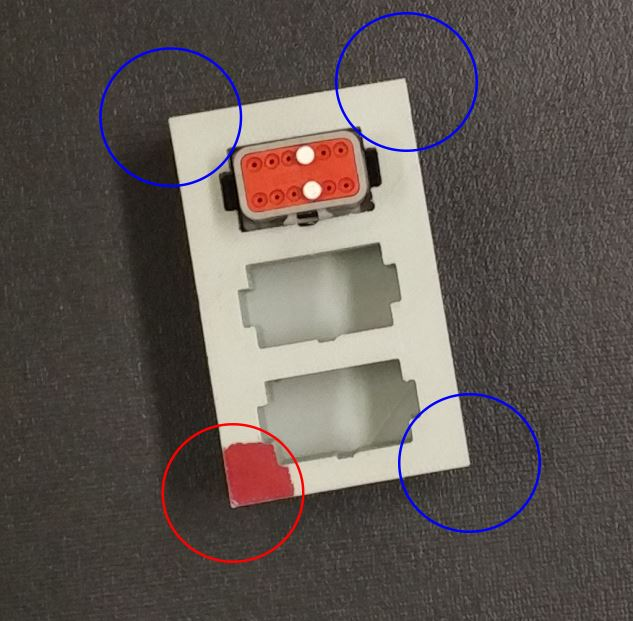
\includegraphics[width=0.5\linewidth]{Redest}
	\caption{Red detection for reference corner}
	\label{fig:Redest}\end{figure}
This reference corner was then used to determine the holding box true angle in relation to the camera. This is required as the angle of the RotatedRect is only in the range 0$^{\circ}$ to -90$^{\circ}$. Shown in  \cref{fig:angleissue}, the RotatedRect is initially a short, wide rectangle at -20$^{\circ}$. However, when rotated by -80$^{\circ}$ the RotatedRect becomes a tall, thin rectangle at -10$^{\circ}$. To rectify this, the index of the reference corner from the list of corners returned from the RotatedRect function was examined, and the true angle was found with an addition of 0, 90$^{\circ}$, 180$^{\circ}$ or 270$^{\circ}$. 

\begin{figure}[h]
\centering
\includegraphics[width=0.7\linewidth]{"angle issue"}
\caption{}
\label{fig:angleissue}
\end{figure}

This orientation process is repeated for the gripper arm, but using the blue and green dots on the gripper fingers. 
	
\section{Pin detection and PinHole Allocation}
With the holding block true angle determine, a copy of the image can be rotated and cropped to be only the holding block. This cropping can be seen in \cref{fig:holdingblockwithdata}.
\begin{figure}[h]
	\centering
	\includegraphics[width=0.4\linewidth]{"holding block with data"}
	\caption{Holding block image, cropped down to only the block, and with all socket overlay shown}
	\label{fig:holdingblockwithdata}
\end{figure}\\
Data on this holding block can now be used for finding the sockets in the holding block. \footnote{At this point, hard coding has been used, however if several holding blocks are used in future development a bar code system will be introduced for identification and CSV extraction use.} This information defines how large the block is in millimetres, so a pixel per millimetre ratio can be found. The block information also defines were the sockets should be (in millimetres), within the block.\\
By using the ratio, and the physical displacement of each socket, a socket object can now be made. Each socket object is passed the holding block image, its pixel starting point within this image, expected hight, and file name for CSV file with pin details. The socket starts by cropping a reference matrix of the block image. Using reference copies, or \textit{shallow copies}, has two main advantages: Firstly, the memory used  and copy execution time is reduced, as the socket's stored \textit{Mat} is only a pointer, not a whole new matrix. Secondly, the socket image can be edited for user feedback, and the original holding block image is effected. This allows only a holding box to be presented to the user with all socket information being shown, rather than loading each socket image separately. An example of this is shown in \cref{fig:holdingblockwithdata}. 



Using its sub-matrix, the socket examines the mean red ratios, as seen for the holding block corner, and determines if a socket is present, or if the socket place is empty, as shown in \cref{fig:fullSock}.
\begin{figure}[h]
\hspace*{-.05\linewidth}
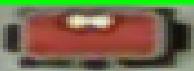
\includegraphics[width=0.5\linewidth]{fullSock}
\hspace*{0.05\linewidth}
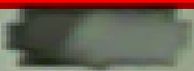
\includegraphics[width=0.5\linewidth]{emptySock}
\caption{Active and empty socket place identified and presented with, respectively, green or red bar above}
\label{fig:fullSock}
\end{figure}\\

Sockets that have been identified as present are then further examined to find the exact area for pin hole mounting. Shown in \cref{fig:sock1} is the original socket image. A threshold function of high red, low green, low blue is then performed, \cref{fig:sock2}. The image is eroded and dilated, \cref{fig:sock3}, and a canny edge detection is conducted, \cref{fig:sock4}. The image is then cropped to fit the resulting contour, \cref{fig:sock5}.\\

\begin{figure}[h]
	\centering
	\begin{subfigure}{0.4\linewidth}
		\centering
		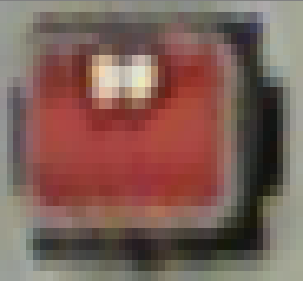
\includegraphics[width=\linewidth]{sock1}
		\subcaption{original sub-matrix}
		\label{fig:sock1}
	\end{subfigure} \hspace{0.1\linewidth}
	\begin{subfigure}{0.4\linewidth}
		\centering
		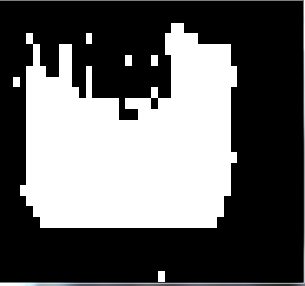
\includegraphics[width=\linewidth]{sock2}
		\subcaption{Post-threshold}
		\label{fig:sock2}
	\end{subfigure}
	\begin{subfigure}{0.4\linewidth}
		\centering
		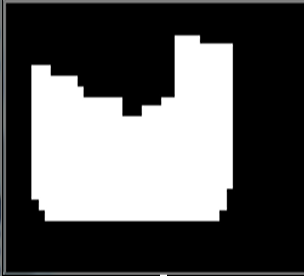
\includegraphics[width=\linewidth]{sock3}
		\subcaption{Small specs removed}
		\label{fig:sock3}
	\end{subfigure}\hspace{0.1\linewidth}
	\begin{subfigure}{0.4\linewidth}
		\centering
		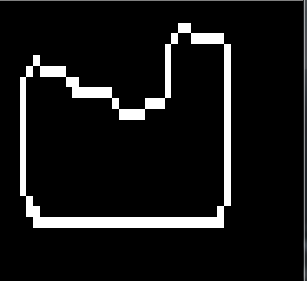
\includegraphics[width=\linewidth]{sock4}
		\subcaption{Edge detection}
		\label{fig:sock4}
	\end{subfigure}
	\begin{subfigure}{0.4\linewidth}
		\centering
		
\includegraphics[width=\linewidth]{sock5}
		\subcaption{Matrix refit to edge of red area}
		\label{fig:sock5}
	\end{subfigure}\hspace{0.1\linewidth}
	\begin{subfigure}{0.4\linewidth}
		\centering
		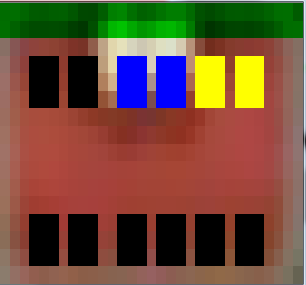
\includegraphics[width=\linewidth]{sock6}
		\subcaption{Pins identifed}
		\label{fig:sock6}
	\end{subfigure}
	\caption{Image processing of socket}
\end{figure}

Using a CSV dataset, the locations of the pins is then assigned. \note{may be able to add stuff here if better res camera allows us to have an extra layer of positioning}
The newly allocated pin hole is examined to find if a pin is present. To do this, the mean value of all three colour channels is compared with the 3 mean channels of the socket, if it is 25\% greater, a (white) pin is determined to be present.\\
A second CSV file then provides information on which pin holes should be filled. The resulting pin layout is shown in \cref{fig:sock6}, black pin holes are not filled, and should not be, blue have already been filled, and yellow still need to be filled.


 \FloatBarrier
\section{Path creation}
workds words words


\chapter{Robotic Arm Control}
\section{Denavit-Hartenberg Algorithm}
\section{Matlab Simulations}
\section{Open ABB}
For this project, a basic parallel port could not be used. As more complex data transfer was required.\\ The parallel port allowed for single bits to be used as flags which triggered the robotic arm to perform action sets. For this project we needed to send specific travel distances. To achieve this, OpenABB (https://github.com/robotics/open_abb) was used. This system has the robotic controller running a basic TCP server via RAPID code. A python script is used on the computer to connect to this server, and send commands. One such command can move the gripper to any point in the arms \hl{range/ field of operations, something like that} by sending the three axis coordinates.\\
This command list was extended by the team to  include gripper control and moving about the x and y axis, while leaving the z value constant. 
An example of the command stack is shown in \cref{fig:comstack1}.

\chapter{Coordination}
As the computer vision was made in c++, and the openABB c++ code requires a full ROS installation, it was instead chosen to implement a python calling system in c++. This interface called a python run-time, and was sent commands via \textit{PyRun_SimpleString}.\\
The command stack was thus extended as shown in \cref{fig:comstack2}

\appendix
\chapter{Initial project request}
\note{get pdf of project request paper}
\end{document}